% Provenance (never printed): see sources/outline_sources.md (Year 1: hotspots and
% mantle plumes; hotspot chains and absolute plate motion; large igneous provinces).
% Hotspot map, pole fit, rates and swell from figdata/bachelor-1/hotspots.py (data
% data/derived/bachelor-1-hotspots.csv, Table 1 of the Morgan and Morgan 2007 electronic
% supplement); exercise and problem values in the Book 3 scratch calculators calc/ch15.py and
% calc/ch15ex.py. "Hotspot" is re-founded from Book 1 (g7 volcanoes), "hotspot track"
% from Book 2 (g11 plate-motions); Book 2 owns the age--distance fit of the Hawaiian
% chain, so this chapter fits the Pacific Euler pole from track directions instead.
\chapter{Hotspots and Intraplate Volcanism}\label{ch:b1:hotspots}

From January 1983, and for decades after, Kilauea, on the island of Hawaii,
erupted almost without a pause from a vent on its east rift zone,
Pu\textquoteleft u~\textquoteleft O\textquoteleft o, pouring out about
\qty{0.12}{km^3} of lava a year. Kilauea stands in the middle of the Pacific plate,
thousands of kilometres from any ridge or trench. To the north-west the
islands of Hawaii are older and older, then they sink below the sea and the
chain goes on as a line of drowned volcanoes for thousands of kilometres more.
Plate tectonics explains volcanoes at plate boundaries; this chapter is about
the ones it does not explain directly, the \omterm{def:b1:hotspots:hotspot}{hotspots}, and about what they tell
us in return: how the plates move over the deep \omterm{def:b1:layered-earth:layers}{mantle}, how much heat and rock
rise from below, and how a few enormous outpourings of lava, the \omterm{def:b1:hotspots:lip}{large igneous
provinces}, were made.
% ledger: pp1801:kilauea-rate

\begin{recall}
A \omterm{def:b1:hotspots:hotspot}{hotspot} feeds volcanoes from deep in the \omterm{def:b1:layered-earth:layers}{mantle} while the plate moves above
it, and the plate carries away a \omterm{def:b1:hotspots:track}{hotspot track} whose volcanoes are older with
distance (Book 1, grade 7; Book 2, grade 11). A plate turning with the \omterm{def:b1:plate-kinematics:euler-pole}{Euler
vector} $\vec\omega$ moves at $\vec v = \vec\omega\times\vec r$, at the speed
$\omega R\sin\Delta$, perpendicular to the \omterm{def:b1:spherical-astronomy:spherical-triangle}{great circle} that joins it to the
pole (\cref{ch:b1:plate-kinematics}); relief is held up by \omterm{def:b1:isostasy-gravity:isostasy}{isostasy}
(\cref{ch:b1:isostasy-gravity}); warm rock is lighter by the fraction
$\alpha\,\Delta T$ (\cref{ch:b1:rifts-ridges-margins}).
\end{recall}

\section{Hotspots and mantle plumes}\label{sec:b1:hotspots:plumes}

\begin{definition}[Hotspot]\label{def:b1:hotspots:hotspot}
A \emph{hotspot}\index{hotspot} is a region of volcanism whose position does
not depend on the plate boundaries, active over tens of millions of years,
and thought to be fed by \omterm{def:b1:layered-earth:layers}{mantle} that is hotter than the \omterm{def:b1:layered-earth:layers}{mantle} around it.
\end{definition}

How many \omterm{def:b1:hotspots:hotspot}{hotspots} there are depends on what one counts. The table of \omterm{def:b1:hotspots:hotspot}{hotspots}
used in this chapter lists 68 of them, but its authors leave out several
features they judge not to record the motion of a plate, and they rate some of
those they keep only as probable. Some \omterm{def:b1:hotspots:hotspot}{hotspots}, among them Hawaii, Iceland and
Réunion, have long, regular tracks and a large output, as a deep source
would; others are small and short-lived. Most \omterm{def:b1:hotspots:hotspot}{hotspot} volcanoes erupt basalt;
where a \omterm{def:b1:hotspots:hotspot}{hotspot} lies beneath a continent, the hot basalt melts the \omterm{def:b1:layered-earth:layers}{crust}, and
the great eruptions turn to rhyolite, as at Yellowstone.
% ledger: mm07:table, data:b3-hotspots, yvo:calderas

\begin{definition}[Mantle plume]\label{def:b1:hotspots:plume}
A \emph{mantle plume}\index{mantle plume} is a column of hot, buoyant \omterm{def:b1:layered-earth:layers}{mantle}
rock that rises from a \omterm{def:b1:heat-budget:boundary-layer}{thermal boundary layer} deep in the \omterm{def:b1:layered-earth:layers}{mantle}. A new plume
has a large, bulbous \emph{head} on a long, narrow \emph{tail}, or conduit; once
the head has spread beneath the \omterm{def:b1:layered-earth:lithosphere}{lithosphere}, the tail goes on feeding melt to
the surface for tens of millions of years.
\end{definition}

The shape comes from the laboratory. In tank experiments of the 1970s, a layer
of light fluid less viscous than the fluid above it rose as a round pocket fed
by a pipe behind it: a mushroom. The head of a \omterm{def:b1:hotspots:plume}{mantle plume} reaching the base
of the \omterm{def:b1:layered-earth:lithosphere}{lithosphere} spreads out and flattens; the pressure falls, and the hot
rock melts in large amounts. Flood basalts fit the picture: their volcanism
lasts some ten million years, but most of their volume is erupted in about a
million years or less, and they often go with the breaking apart of a
continent (\cref{sec:b1:hotspots:lips}).
% ledger: hist:plumes (Whitehead and Luther 1975), cr03:summary

\begin{omfigure}
\begin{tikzpicture}[font=\scriptsize,
  lbl/.style={fill=white, fill opacity=0.8, text opacity=1, inner sep=1pt, align=center}]
% ---- panel (a): the head arrives ----
\begin{scope}
\clip (0,-5) rectangle (6.4,1.3);
\fill[orange!12] (0,-5) rectangle (6.4,0);
\fill[omSea!45] (0,0) rectangle (6.4,0.55);
\fill[omLithBasalt!55] (0,0) rectangle (6.4,-0.9);
% flood basalt: a stack of flat flows on the sea floor
\fill[black!55] (2.5,0) -- (2.7,0.32) -- (6.1,0.32) -- (6.3,0) -- cycle;
\foreach \y in {0.08,0.16,0.24} \draw[white!70!black, line width=0.3pt] (2.62,\y) -- (6.18,\y);
% plume: tail and flattened head
\fill[red!40] (4.25,-5) -- (4.25,-1.7) -- (4.55,-1.7) -- (4.55,-5) -- cycle;
\fill[red!40] (4.4,-1.45) ellipse[x radius=1.9, y radius=0.55];
\draw[red!60!black, line width=0.4pt] (4.25,-5) -- (4.25,-1.95) (4.55,-5) -- (4.55,-1.95);
\draw[red!60!black, line width=0.4pt] (4.4,-1.45) ellipse[x radius=1.9, y radius=0.55];
% melt rising through the plate
\foreach \x in {3.2,3.9,4.6,5.3}
  \draw[red!75!black, line width=0.6pt, decorate, decoration={snake, amplitude=0.6pt, segment length=3pt}] (\x,-1.1) -- (\x,0.05);
\end{scope}
\draw[black!70] (0,-5) rectangle (6.4,1.3);
\node[lbl, anchor=north west] at (0.1,1.25) {(a) the head arrives};
\node[lbl, anchor=west] at (0.1,-0.45) {lithosphere};
\node[lbl, anchor=west] at (0.1,0.3) {sea};
\node[lbl, anchor=south] at (4.4,0.62) {flood basalt (LIP)};
\node[lbl, anchor=east] (ph) at (1.9,-1.75) {plume head};
\draw[black!70] (ph.east) -- (2.7,-1.6);
\node[lbl, anchor=east] at (4.1,-3.6) {plume tail};
\node[lbl, anchor=west] at (0.1,-4.6) {mantle};
% ---- panel (b): the plate has moved on ----
\begin{scope}[xshift=6.8cm]
\begin{scope}
\clip (0,-5) rectangle (6.4,1.3);
\fill[orange!12] (0,-5) rectangle (6.4,0);
\fill[omSea!45] (0,0) rectangle (6.4,0.55);
\fill[omLithBasalt!55] (0,0) rectangle (6.4,-0.9);
% the flood basalt, carried away to the left
\fill[black!55] (-0.9,0) -- (-0.7,0.32) -- (1.0,0.32) -- (1.2,0) -- cycle;
\foreach \y in {0.08,0.16,0.24} \draw[white!70!black, line width=0.3pt] (-0.8,\y) -- (1.08,\y);
% the chain: older volcanoes to the left, lower (they sank as the plate cooled)
\fill[black!35] (1.45,0) -- (1.75,0.2) -- (2.05,0) -- cycle;
\fill[black!38] (2.15,0) -- (2.5,0.3) -- (2.85,0) -- cycle;
\fill[black!42] (2.95,0) -- (3.35,0.42) -- (3.75,0) -- cycle;
\fill[black!65] (3.95,0) -- (4.45,0.95) -- (4.55,0.97) -- (5.05,0) -- cycle;
\fill[red!70!black] (4.43,0.93) -- (4.57,0.95) -- (4.5,1.12) -- cycle;
% the plume tail, still in place, and a small spread of hot rock under the plate
\fill[red!40] (4.35,-5) -- (4.35,-1.1) -- (4.65,-1.1) -- (4.65,-5) -- cycle;
\fill[red!40] (4.5,-1.05) ellipse[x radius=0.75, y radius=0.2];
\draw[red!60!black, line width=0.4pt] (4.35,-5) -- (4.35,-1.2) (4.65,-5) -- (4.65,-1.2);
\draw[red!75!black, line width=0.6pt, decorate, decoration={snake, amplitude=0.6pt, segment length=3pt}] (4.5,-0.95) -- (4.5,0.8);
\end{scope}
\draw[black!70] (0,-5) rectangle (6.4,1.3);
\node[lbl, anchor=north west] at (0.1,1.25) {(b) much later};
\draw[->, line width=1pt] (3.2,-0.45) -- (1.2,-0.45) node[midway, above=1pt, lbl] {plate motion};
\node[lbl, anchor=south] at (0.55,0.38) {the LIP};
\node[lbl, anchor=south] at (2.7,0.62) {older, extinct};
\node[lbl, anchor=west] at (5.0,0.95) {active\\volcano};
\node[lbl, anchor=east] at (4.2,-3.6) {plume tail};
\node[lbl, anchor=west] at (4.75,-2.6) {stays in\\the mantle};
\end{scope}
\end{tikzpicture}
\par\smallskip{\small The plume model of a \omterm{def:b1:hotspots:hotspot}{hotspot} (schematic, not to scale).
(a)~A new plume: its head flattens beneath the \omterm{def:b1:layered-earth:lithosphere}{lithosphere} and melts as it
decompresses, and a flood basalt, a \omterm{def:b1:hotspots:lip}{large igneous province}, is erupted in a
few million years or less. (b)~Tens of millions of years later the plate has
carried the province away; the narrow tail still feeds an active volcano, and
the volcanoes it built before are extinct, older with distance, and lower,
for they sink with the cooling plate.}
\label{fig:b1:hotspots:plume}
\end{omfigure}

What is the evidence for plumes? First, the age-progressive chains themselves,
which a narrow source fixed beneath a moving plate explains at once
(\cref{sec:b1:hotspots:tracks}). Second, the lavas of some \omterm{def:b1:hotspots:hotspot}{hotspots} carry
unusually high ratios of the light to the heavy isotope of helium, read as the
signature of a deep reservoir that has kept some of the gas the Earth was made
with. Third, the sources are hot: the lavas of ocean islands and plateaus point
to \omterm{def:b1:layered-earth:layers}{mantle} 200 to \qty{300}{\celsius} hotter than the \omterm{def:b1:layered-earth:layers}{mantle} beneath the ridges,
whose potential temperature lies between 1280 and \qty{1400}{\celsius}. Fourth,
seismic images of the \omterm{def:b1:layered-earth:layers}{mantle}: beneath Hawaii, a network of seismometers on the
sea floor and on the islands imaged a hot column reaching down into the lower
\omterm{def:b1:layered-earth:layers}{mantle}, and a model of the whole \omterm{def:b1:layered-earth:layers}{mantle} built in 2015 from complete seismic
waveforms shows broad, roughly vertical columns beneath many of the major
\omterm{def:b1:hotspots:hotspot}{hotspots}, rising from the \omterm{def:b1:layered-earth:discontinuity}{core--mantle boundary} to about \qty{1000}{km} below
the surface; beneath Hawaii, Iceland and Samoa they are rooted in patches of
very low wave speed at the base of the \omterm{def:b1:layered-earth:layers}{mantle}. How such images are made belongs
to the Year 3 volume.
% ledger: herzberg:tp, wolfe:hawaii, fr15:plumes

None of this is a proof, and the debate is alive. In the plate hypothesis,
defended by Gillian Foulger and James Natland among others, \omterm{def:b1:hotspots:hotspot}{hotspot} volcanism
is not especially hot and needs no deep plume: it is a by-product of plate
tectonics, fed from shallow sources where the \omterm{def:b1:layered-earth:lithosphere}{lithosphere} is stretched or
cracked. Their opponents hold that the evidence for at least some deep plumes
is strong, though the seismic images are not yet sharp enough to settle it; and
the \omterm{def:b1:hotspots:hotspot}{hotspots}, as the next section shows, are not quite fixed.
% ledger: fn03:plate-hypothesis, tarduno:emperor

\section{Hotspot tracks and the motion of the plates}\label{sec:b1:hotspots:tracks}

\begin{definition}[Hotspot track; age progression]\label{def:b1:hotspots:track}
A \emph{hotspot track}\index{hotspot track} is the line of volcanoes, seamounts
and volcanic ridges that a plate carries away from a \omterm{def:b1:hotspots:hotspot}{hotspot} as it moves over
it. Its \emph{age progression}\index{age progression} is the regular increase
of the ages of its volcanoes with the distance from the active one. The
\emph{direction} of a track at the \omterm{def:b1:hotspots:hotspot}{hotspot} is the \omterm{def:b1:spherical-astronomy:horizontal}{azimuth}, measured from north,
towards which its young part runs away from the \omterm{def:b1:hotspots:hotspot}{hotspot}.
\end{definition}

If the \omterm{def:b1:hotspots:hotspot}{hotspots} stay fixed in the deep \omterm{def:b1:layered-earth:layers}{mantle}, a track records the motion of the
plate over the deep \omterm{def:b1:layered-earth:layers}{mantle}: its direction is that of the plate's velocity at
the \omterm{def:b1:hotspots:hotspot}{hotspot}, and its \omterm{def:b1:hotspots:track}{age progression} gives the speed. Book 2, grade 11, read the
speed of the Pacific plate from the ages of the Hawaiian volcanoes. The
directions alone already say more: they give the \omterm{def:b1:plate-kinematics:euler-pole}{Euler pole}.

\begin{proposition}[The Euler pole from two tracks]\label{prop:b1:hotspots:two-tracks}
Let a \omterm{def:b1:plate-kinematics:rigid-plate}{rigid plate} move over two fixed \omterm{def:b1:hotspots:hotspot}{hotspots} at the positions $\vec r_1$ and
$\vec r_2$, and let $\vec t_1$ and $\vec t_2$ be the horizontal unit vectors
along their tracks. If $\vec t_1$ and $\vec t_2$ are not parallel, the \omterm{def:b1:plate-kinematics:euler-pole}{Euler
vector} of the plate relative to the \omterm{def:b1:hotspots:hotspot}{hotspots} is parallel to
$\vec t_1\times\vec t_2$, and its pole is the unit vector
\[
  \vec p = \pm\frac{\vec t_1\times\vec t_2}{\lVert\vec t_1\times\vec t_2\rVert},
\]
with the sign for which $(\vec p\times\vec r_1)\cdot\vec t_1 > 0$.
\end{proposition}

\begin{proof}
At each \omterm{def:b1:hotspots:hotspot}{hotspot} the plate moves with $\vec v_i = \vec\omega\times\vec r_i$
(\cref{thm:b1:plate-kinematics:velocity}), and the track points along it:
$\vec v_i = v_i\vec t_i$ with $v_i > 0$. A cross product is perpendicular to its
factors, so $\vec\omega\cdot\vec t_i = 0$ for $i = 1, 2$: $\vec\omega$ is
perpendicular to two vectors that are not parallel, hence parallel to their
cross product. Of the two unit vectors along it, the pole is the one about
which the rotation is anticlockwise, that is, the one for which
$\vec p\times\vec r_1$ points the way the plate moves at the first \omterm{def:b1:hotspots:hotspot}{hotspot},
along $+\vec t_1$.
\end{proof}

To use the proposition one needs, at a point of \omterm{def:b1:spherical-astronomy:geographic}{latitude} $\varphi$ and \omterm{def:b1:spherical-astronomy:geographic}{longitude}
$\lambda$, the unit vectors pointing east and north,
\[
  \vec e = (-\sin\lambda,\ \cos\lambda,\ 0),\qquad
  \vec n = (-\sin\varphi\cos\lambda,\ -\sin\varphi\sin\lambda,\ \cos\varphi),
\]
in the axes of \cref{ch:b1:plate-kinematics} ($x$ towards \ang{0}\,N
\ang{0}\,E, $y$ towards \ang{0}\,N \ang{90}\,E, $z$ towards the north pole). A
track of \omterm{def:b1:spherical-astronomy:horizontal}{azimuth} $\theta$ runs along $\vec t = \sin\theta\,\vec e +
\cos\theta\,\vec n$. With the Hawaiian track, \omterm{def:b1:spherical-astronomy:horizontal}{azimuth} \ang{304}, and the
Louisville track, \omterm{def:b1:spherical-astronomy:horizontal}{azimuth} \ang{316}, the proposition puts the pole of the
Pacific plate at \ang{56.2}\,S, \ang{124.0}\,E (the weekend problem does the
computation).
% values (hotspots.py): two_pole_lat -56.1805, two_pole_lon 124.008; ledger: data:b3-hotspots

Two tracks determine the pole but cannot test it. Many tracks over-determine
it, and the misfit says whether the \omterm{def:b1:hotspots:hotspot}{hotspots} behave as a fixed frame. W. Jason
Morgan, who proposed the deep plumes, and Jason Phipps Morgan compiled in 2007
a table of 68 \omterm{def:b1:hotspots:hotspot}{hotspots}, with, where they could be measured, the direction of
the track and the speed of the plate over the \omterm{def:b1:hotspots:hotspot}{hotspot}, each with its
uncertainty and a weight for its reliability; a \omterm{def:b1:hotspots:hotspot}{hotspot} under two plates, as
Iceland is, has a line for each. Fifteen weighted tracks lie on the Pacific
plate, thirteen of them with a speed.
% ledger: data:b3-hotspots, mm07:table; values (hotspots.py): n_all 71 rows, n_pacific 15, n_rated 13

\begin{method}[Fitting an Euler pole and a rate to hotspot tracks]\label{met:b1:hotspots:pole-fit}
Given, for $N$ \omterm{def:b1:hotspots:hotspot}{hotspots} on one plate, the positions, the track directions
$\theta_i \pm \sigma_i$ with weights $w_i$, and for some of them the speeds
$v_i$:
\begin{enumerate}
  \item For a trial pole $\vec p$, compute at each \omterm{def:b1:hotspots:hotspot}{hotspot} the direction of
        $\vec p\times\vec r_i$, the \omterm{def:b1:spherical-astronomy:horizontal}{azimuth} $\hat\theta_i$ of the motion it
        predicts (\cref{prop:b1:plate-kinematics:speed}).
  \item Form the misfit $S(\vec p) = \sum_i w_i\bigl((\hat\theta_i -
        \theta_i)/\sigma_i\bigr)^2$, each difference brought between
        \ang{-180} and \ang{180}.
  \item Search for the pole that minimises $S$: on a grid of the whole sphere,
        then on a finer grid around the best point.
  \item With the pole found, compute for each \omterm{def:b1:hotspots:hotspot}{hotspot} with a speed its angular
        distance $\Delta_i$ to the pole and $x_i = R\sin\Delta_i$. The speeds
        should be $v_i = \omega x_i$: the least-squares rate is
        \[
          \omega = \frac{\sum_i x_i v_i}{\sum_i x_i^2},
        \]
        since $\frac{\mathrm d}{\mathrm d\omega}\sum_i (v_i - \omega x_i)^2 =
        -2\sum_i x_i(v_i - \omega x_i)$ vanishes there.
  \item Judge the fit: if the \omterm{def:b1:hotspots:hotspot}{hotspots} were fixed and the uncertainties
        honest, $S$ would be close to the number of directions less two (the
        two coordinates of the pole fitted).
\end{enumerate}
\end{method}

For the fifteen Pacific tracks the method gives the pole \ang{63.8}\,S,
\ang{112.5}\,E, about \ang{10} from the two-track pole, and from the thirteen
speeds the rate $\omega = \qty{0.92}{\degree\per\Myr}$. At Hawaii, \ang{108.0}
from the pole, the fit predicts a motion towards \ang{298} at
\qty{97}{mm.yr^{-1}}; Morgan and Morgan list $\ang{304}\pm\ang{3}$ and
\qty[uncertainty-mode=separate]{92 \pm 3}{mm.yr^{-1}}. The misfit $S$ is 39
where fixed \omterm{def:b1:hotspots:hotspot}{hotspots} with honest uncertainties would give about 13, and the
speeds scatter about the line by \qty{16}{mm.yr^{-1}} (root mean square): the
Pacific \omterm{def:b1:hotspots:hotspot}{hotspots} form a reference frame good to a few degrees and a few
centimetres a year, not better.
% values (hotspots.py): pole_lon 112.48, pole_lat -63.78, chi2 38.7829, omega_deg_myr 0.920609,
% hawaii_delta 107.998, hawaii_pred_az 297.656, hawaii_pred_rate 97.3581, rms_rate 15.966;
% angle between the two poles 9.5 deg (calc/ch15.py); ledger: data:b3-hotspots

The best-known test of the fixed frame is the bend of the Hawaiian--Emperor
chain. The Hawaiian limb runs north-west; the Emperor seamounts run almost
north, to Meiji Guyot, more than 81 million years old, which is about to go
down at the junction of the Kuril--Kamchatka and Aleutian trenches. Was the
bend a change in the motion of the plate? The magnetisation of the Emperor
lavas, measured on cores drilled from the seamounts, records the \omterm{def:b1:spherical-astronomy:geographic}{latitude} at
which each one cooled (the method belongs to the Year 3 volume): they formed
farther north than Hawaii is today, and between 81 and 47 million years ago the
\omterm{def:b1:hotspots:hotspot}{hotspot} itself moved south at more than \qty{40}{mm} a year. Much of the
Emperor chain records the \omterm{def:b1:hotspots:hotspot}{hotspot}, not the plate. Yet the plate changed too:
new ages place the start of the bend near Kimmei Seamount, about 50 million
years ago, when the spreading ridges of the Pacific were realigned. The plume
may even be older than the chain: the head that first fed it is thought to
have made a plateau about 100 million years ago, which went down a trench 20
to 30 million years ago and now lies about \qty{810}{km} deep beneath
Siberia, west of the Sea of Okhotsk.
% ledger: tarduno:emperor, sharp:bend, wei:plume-head

\begin{omfigure}
\begin{tikzpicture}
\begin{axis}[omrecord, width=0.78\linewidth, height=6.2cm, xmin=0, xmax=7000, ymin=0, ymax=160,
  xlabel={$R\sin\Delta$, distance from the axis of rotation (\unit{km})},
  ylabel={speed over the hotspot (\unit{mm.yr^{-1}})},
  xticklabel style={/pgf/number format/set thousands separator={}},
  legend style={font=\scriptsize, at={(0.03,0.97)}, anchor=north west, cells={anchor=west}}]
% computed in figdata/bachelor-1/hotspots.py; ledger: data:b3-hotspots; values: omega_deg_myr 0.920609
\addplot[only marks, mark=*, mark size=1.5pt, omDef, error bars/.cd, y dir=both, y explicit]
  table[x=x, y=rate, y error=srate] {figdata/out/bachelor-1-hotspots-rates.dat};
\addlegendentry{Pacific hotspots}
\addplot[black, densely dashed, line width=0.7pt] table[x=x, y=rate] {figdata/out/bachelor-1-hotspots-rates-fit.dat};
\addlegendentry{$\omega R\sin\Delta$, $\omega = \ang{0.92}$ per million years}
\draw[black!60] (axis cs:6060,90) -- (axis cs:6550,55) node[font=\scriptsize, anchor=north, black] {Hawaii};
\node[font=\scriptsize, anchor=north west] at (axis cs:4880,64) {Louisville};
\node[font=\scriptsize, anchor=west] at (axis cs:3960,43) {Cobb};
\node[font=\scriptsize, anchor=east] at (axis cs:3570,40) {Bowie};
\end{axis}
\end{tikzpicture}
\par\smallskip{\small The speeds of the Pacific plate over thirteen of its
\omterm{def:b1:hotspots:hotspot}{hotspots}, with their uncertainties, against the distance of each \omterm{def:b1:hotspots:hotspot}{hotspot} from
the axis of rotation through the fitted pole. A \omterm{def:b1:plate-kinematics:rigid-plate}{rigid plate} turning about that
pole puts them on a line through the origin; the least-squares line gives
$\omega = \qty{0.92}{\degree\per\Myr}$. Most \omterm{def:b1:hotspots:hotspot}{hotspots} lie 6000 to
\qty{6400}{km} from the axis, where the speed is nearly the same; the scatter
there, larger than the error bars, shows the limits of a fixed frame. Data:
W.~J. and J.~P. Morgan (2007), Table~1 of their electronic supplement.}
\label{fig:b1:hotspots:rates}
\end{omfigure}

\begin{omfigure}
\begin{tikzpicture}
\begin{axis}[ommap, width=0.96\linewidth, xtick={-180,-90,...,180}, ytick={-60,0,60},
  legend style={font=\scriptsize, at={(0.01,0.02)}, anchor=south west, cells={anchor=west}}]
% computed in figdata/bachelor-1/hotspots.py; ledger: data:b3-hotspots, data:ne-land, data:pb2002
\addplot[fill=omLithAlluv, draw=black!45, line width=0.2pt, forget plot] table {figdata/out/shared-geo-land.dat};
\addplot[omRidge, line width=0.5pt, forget plot] table {figdata/out/shared-geo-ridge.dat};
\addplot[omRidge!70!black, line width=0.5pt, forget plot] table {figdata/out/shared-geo-transform.dat};
\addplot[omTrench, line width=0.5pt, forget plot] table {figdata/out/shared-geo-subduction.dat};
\addplot[black!65, line width=0.5pt, forget plot] table {figdata/out/shared-geo-collision.dat};
\addplot[black, line width=0.7pt, -{Stealth[length=3.5pt]}, quiver={u=\thisrow{dx}, v=\thisrow{dy}}, forget plot]
  table[x=lon, y=lat] {figdata/out/bachelor-1-hotspots-map-arrows.dat};
\addplot[only marks, mark=*, mark size=1.3pt, draw=black, fill=orange!90!red] table {figdata/out/bachelor-1-hotspots-map-hs.dat};
\addlegendentry{hotspot}
\addplot[only marks, mark=star, mark size=3.2pt, line width=0.8pt, omDef] table {figdata/out/bachelor-1-hotspots-map-pole.dat};
\addlegendentry{Euler pole of the Pacific plate}
\draw[black, line width=0.7pt, -{Stealth[length=3.5pt]}] (axis cs:-40,-80) -- (axis cs:-25,-80);
\node[font=\scriptsize, anchor=west, fill=white, fill opacity=0.75, text opacity=1, inner sep=1pt]
  at (axis cs:-23,-80) {\qty{10}{cm} a year};
\node[font=\scriptsize, anchor=north, fill=white, fill opacity=0.75, text opacity=1, inner sep=1pt] at (axis cs:-150,16) {Hawaii};
\node[font=\scriptsize, anchor=north, fill=white, fill opacity=0.75, text opacity=1, inner sep=1pt] at (axis cs:-140.6,-56) {Louisville};
\node[font=\scriptsize, anchor=south, fill=white, fill opacity=0.75, text opacity=1, inner sep=1pt] at (axis cs:-100,49) {Yellowstone};
\node[font=\scriptsize, anchor=south, fill=white, fill opacity=0.75, text opacity=1, inner sep=1pt] at (axis cs:-17.3,66) {Iceland};
\node[font=\scriptsize, anchor=north, fill=white, fill opacity=0.75, text opacity=1, inner sep=1pt] at (axis cs:55.7,-23.5) {Réunion};
\end{axis}
\end{tikzpicture}
\par\smallskip{\small The 68 \omterm{def:b1:hotspots:hotspot}{hotspots} of W.~J. and J.~P. Morgan (2007). Arrows:
the motion of the plate over each \omterm{def:b1:hotspots:hotspot}{hotspot} where it was measured, along the
direction of the track and with a length proportional to the speed (scale at
bottom, south of the Atlantic); where a \omterm{def:b1:hotspots:hotspot}{hotspot} lies under two plates, as Iceland does, both are
drawn. The star is the \omterm{def:b1:plate-kinematics:euler-pole}{Euler pole} of the Pacific plate relative to the
\omterm{def:b1:hotspots:hotspot}{hotspots}, fitted to the fifteen Pacific tracks by
\cref{met:b1:hotspots:pole-fit}: the Pacific arrows turn about it. Plate
boundaries: PB2002 (red: ridges; dark red: transforms; blue: subduction zones;
grey: collision zones).}
\label{fig:b1:hotspots:map}
\end{omfigure}


\omterm{def:b1:hotspots:track}{Hotspot tracks} also cross continents. As the North American plate moved
south-west over the Yellowstone \omterm{def:b1:hotspots:hotspot}{hotspot}, a chain of great calderas formed,
older and older towards the south-west along the Snake River Plain. At its
far end, on the border of Nevada and Oregon, the McDermitt caldera, some
\qty{40}{km} across, collapsed 16.4 million years ago in an eruption of about
\qty{1000}{km^3}. At Yellowstone itself, the first of three caldera-forming
eruptions, 2.1 million years ago, released some \qty{2400}{km^3} of magma and
left a caldera more than \qty{100}{km} across; the last, 640\,000 years ago,
made the present Yellowstone Caldera, \qty{55}{km} by 80. Since 10 million
years ago the onset of the caldera eruptions has moved north-east at
$\qty[uncertainty-mode=separate]{2.9 \pm 0.5}{cm}$ a year, and Morgan and
Morgan give the plate a speed of
\qty[uncertainty-mode=separate]{26 \pm 5}{mm.yr^{-1}} over the \omterm{def:b1:hotspots:hotspot}{hotspot}, towards
\ang{235}; the older calderas, as \cref{exo:b1:hotspots:8} shows, moved
faster.
% ledger: henry:mcdermitt, yvo:calderas, pm90:track, data:b3-hotspots

\section{Swells, buoyancy and the supply of magma}\label{sec:b1:hotspots:swells}

Hawaii does not stand on ordinary ocean floor. In 1953 Robert Dietz and
William Menard described the broad rise of the sea floor on which the islands
sit, the Hawaiian swell. The swell is not compensated by thick \omterm{def:b1:layered-earth:layers}{crust}: it is
held up from below by the hot, light rock of the plume as it spreads beneath
the plate, a \emph{dynamic} support. Over the swell the \omterm{def:b1:heat-budget:heat-flow}{heat flow} at the
surface is at most 5 to \qty{10}{mW.m^{-2}} higher than around it, and perhaps
not higher at all.
% ledger: hist:plumes (Dietz and Menard 1953), vh89:swell-heat

Its shape can be read from the global grid of depths. Take sections across the
track, perpendicular to its direction, every \qty{50}{km} from the \omterm{def:b1:hotspots:hotspot}{hotspot} to
\qty{1000}{km} downstream; at each distance from the axis of the chain, the
median of the depths on these sections gives a profile that keeps the swell and
smooths away the single volcanoes (the figure after the next proposition). Far from the chain, 1000 to
\qty{1500}{km} on either side, the floor lies at \qty{5274}{m}. Close to it,
the islands and seamounts stand up to \qty{3}{km} higher; replace them by a
straight line across the \qty{300}{km} of the chain, and what remains is the
swell: about \qty{690}{m} high at most, a few hundred kilometres wide on each
side, with a cross-section of $A \approx \qty{4.8e8}{m^2}$ above the far
floor.
% values (hotspots.py): swell_ref -5273.64, swell_height 690.636, swell_area_m2 4.82786e8;
% ledger: data:etopo1, data:b3-hotspots (Hawaii 19.0 N 155.2 W, track 304)

The swell measures the plume. It is carried away with the plate and remade
over the \omterm{def:b1:hotspots:hotspot}{hotspot}, so the plume must supply buoyancy as fast as the plate takes
it away.

\begin{proposition}[Buoyancy flux of a plume]\label{prop:b1:hotspots:buoyancy}
Let a plate move at the speed $v$ over a \omterm{def:b1:hotspots:hotspot}{hotspot}, and let the swell around the
track have the cross-section $A$ above the floor far from it, the swell being in
isostatic equilibrium (\cref{def:b1:isostasy-gravity:isostasy}) and supported
by light rock carried along with the plate. Then the plume delivers mass
deficit, its \emph{buoyancy flux}, at the rate
\[
  B = (\rho_m - \rho_w)\,A\,v ,
\]
where $\rho_m$ is the density of the \omterm{def:b1:layered-earth:layers}{mantle} and $\rho_w$ that of sea water.
\end{proposition}

\begin{proof}
Consider a column through the swell, where the floor is raised by $h$, and a
column far from it, both down to a \omterm{def:b1:isostasy-gravity:isostasy}{compensation depth}. Between the two floors
the far column holds water and the swell column rock: the swell column has the
extra mass $(\rho_m - \rho_w)h$ per unit area there. Equal masses above the
\omterm{def:b1:isostasy-gravity:isostasy}{compensation depth} (\cref{prop:b1:isostasy-gravity:equal-mass}) require a mass
deficit of the same size lower down in the swell column, in the light plume
rock. Across the track, the deficit per unit length of track is
$\int(\rho_m - \rho_w)h\,\mathrm dy = (\rho_m - \rho_w)A$. In a time
$\mathrm dt$ the plate carries a length $v\,\mathrm dt$ of swell downstream,
with its deficit, and the swell over the \omterm{def:b1:hotspots:hotspot}{hotspot} keeps its shape: the plume
must supply the deficit $(\rho_m - \rho_w)A\,v\,\mathrm dt$.
\end{proof}

\begin{omfigure}
\begin{tikzpicture}
\begin{axis}[omrecord, width=0.86\linewidth, height=6cm, xmin=-1500, xmax=1500, xtick={-1500,-1000,...,1500}, ymin=-6000, ymax=-1000,
  xlabel={distance across the Hawaiian chain, south-west to north-east (\unit{km})},
  ylabel={depth of the sea floor (\unit{m})},
  xticklabel style={/pgf/number format/set thousands separator={}},
  yticklabel style={/pgf/number format/set thousands separator={}},
  legend style={font=\scriptsize, at={(0.99,0.97)}, anchor=north east, cells={anchor=west}}]
% computed in figdata/bachelor-1/hotspots.py; ledger: data:etopo1, data:b3-hotspots
\addplot[name path=hi, draw=none, forget plot] table[x=d, y=q75] {figdata/out/bachelor-1-hotspots-swell.dat};
\addplot[name path=lo, draw=none, forget plot] table[x=d, y=q25] {figdata/out/bachelor-1-hotspots-swell.dat};
\addplot[omSea!60, forget plot] fill between[of=hi and lo];
\addplot[black, line width=0.8pt] table[x=d, y=med] {figdata/out/bachelor-1-hotspots-swell.dat};
\addlegendentry{median depth}
\addplot[omDef, line width=0.9pt, densely dashed] table[x=d, y=swell] {figdata/out/bachelor-1-hotspots-swell-ref.dat};
\addlegendentry{swell, chain removed}
\addplot[black!60, densely dotted, line width=0.7pt] table[x=d, y=ref] {figdata/out/bachelor-1-hotspots-swell-ref.dat};
\addlegendentry{reference, 1000 to \qty{1500}{km} out}
\node[font=\scriptsize, anchor=south] at (axis cs:-330,-3300) {the chain};
\end{axis}
\end{tikzpicture}
\par\smallskip{\small The Hawaiian swell. Each point is the median of 21 depths,
taken on sections across the chain every \qty{50}{km} from the \omterm{def:b1:hotspots:hotspot}{hotspot} to
\qty{1000}{km} downstream, at the same distance from the axis of the chain;
the shaded band holds the middle half of the 21 depths. The chain itself, a
narrow spike, is replaced by a straight line (dashed) to leave the swell, about
\qty{690}{m} above the floor far from the chain (dotted). Depths: ETOPO1,
sampled at one degree.}
\label{fig:b1:hotspots:swell}
\end{omfigure}

A buoyancy flux is a flow of missing mass: it counts how fast the plume brings
light rock up. What makes the rock light is heat, so the buoyancy flux is also
a heat flux.

\begin{proposition}[Heat carried by a plume]\label{prop:b1:hotspots:heat}
If the rock of a plume is $\Delta T$ hotter than the \omterm{def:b1:layered-earth:layers}{mantle} around it, with
the coefficient of thermal expansion $\alpha$ and the specific heat capacity
$c_p$, its buoyancy flux $B$ and the excess heat it carries, $Q$, satisfy
\[
  Q = \frac{c_p}{\alpha}\,B ,
\]
whatever $\Delta T$.
\end{proposition}

\begin{proof}
Let the plume carry the mass $\Phi$ of hot rock per unit time. Each unit
volume of it is lighter than the \omterm{def:b1:layered-earth:layers}{mantle} by $\rho_m\alpha\,\Delta T$, which is,
to first order, a mass deficit $\alpha\,\Delta T$ per unit mass: $B =
\alpha\,\Delta T\,\Phi$. Each unit mass carries the excess heat
$c_p\,\Delta T$: $Q = c_p\,\Delta T\,\Phi$. Dividing, $\Delta T$ and $\Phi$
cancel.
\end{proof}

For Hawaii, with $\rho_m - \rho_w = \qty{2300}{kg.m^{-3}}$, $A =
\qty{4.83e8}{m^2}$ and $v = \qty{92}{mm.yr^{-1}} = \qty{2.92e-9}{m.s^{-1}}$,
\[
  B = 2300\times\num{4.83e8}\times\num{2.92e-9} \approx \qty{3240}{kg.s^{-1}}:
\]
the plume brings up about three tonnes of missing mass every second. Rocks
store 2 to \qty{3}{MJ} per cubic metre and per kelvin; with \qty{3}{MJ} the
\omterm{def:b1:layered-earth:layers}{mantle}, of density \qty{3300}{kg.m^{-3}}, has
$c_p \approx \qty{910}{J.kg^{-1}.K^{-1}}$;
with $\alpha = \qty{3.2e-5}{K^{-1}}$,
\[
  Q = \frac{910}{\num{3.2e-5}}\times3240 \approx \qty{9.2e10}{W},
\]
\qty{0.2}{\percent} of the \qty{47}{TW} that leave the whole Earth. The
strongest plume on Earth is a small item in the planet's heat budget
(\cref{ch:b1:heat-budget}); most of the heat leaves through the ocean floor
made at the ridges.
% values (hotspots.py): swell_B_kg_s 3237.18; Q = 9.1951e10 W (calc/ch15.py);
% ledger: data:b3-hotspots (92 mm/yr), delaney86:properties (Book 2 row), parsons:plate-model (alpha), dd10:total

The magma tells the same story. Since 81 million years ago the \omterm{def:b1:hotspots:hotspot}{hotspot} has
built the Hawaiian--Emperor chain, about two million cubic kilometres of
basalt once the sinking of the plate beneath its load is counted, an average of
\qty{0.025}{km^3} a year; but about a quarter of it was erupted in the last six
million years, and Kilauea alone is supplied today with about \qty{0.1}{km^3}
of magma a year. Mauna Loa, the largest volcano of the islands, holds some
\qty{74000}{km^3}, and Mauna Kea, its neighbour, rises \qty{4205}{m} above the
sea. Yet the ridges make about \qty{21}{km^3} of ocean \omterm{def:b1:layered-earth:layers}{crust} a year, two
hundred times the present supply of Kilauea.
% ledger: pp1801:chain-volume, pp1801:kilauea-supply, pp1801:volumes, data:pb2002 (ridge_budget.py 21.36 km3/yr)

\begin{omfigure}
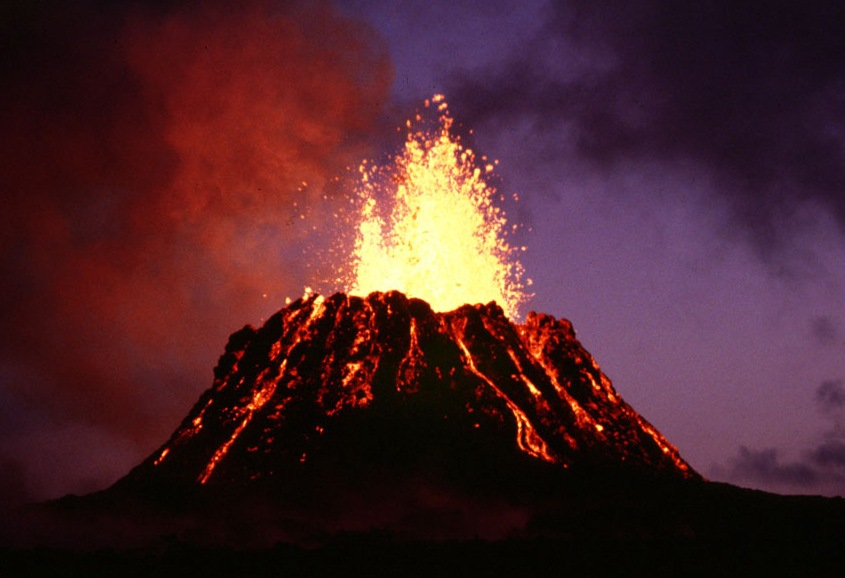
\includegraphics[width=0.55\linewidth]{images/book3/b1-puu-oo-1983.jpg}
\par\smallskip{\small A lava fountain on the Pu\textquoteleft
u~\textquoteleft O\textquoteleft o cone, on the east rift zone of Kilauea,
29 June 1983, in the first year of an eruption that went on for decades:
basaltic lava, hot and runny, thrown up in a jet and falling back around the
vent. Photograph: G.~E.~Ulrich, U.S. Geological Survey, public domain
(Wikimedia Commons).}
\label{fig:b1:hotspots:puu-oo}
\end{omfigure}
% ledger: commons:puu-oo, pp1801:kilauea-rate

\begin{history}[A fixed frame for the plates]
In 1963 John Tuzo Wilson explained the Hawaiian Islands, older and older along
a line, by a source of lava held in the slow core of a \omterm{def:b1:layered-earth:layers}{mantle} convection cell,
while the faster upper part of the cell carried the sea floor over it.
In 1971 and 1972 W. Jason Morgan made that source a plume, about
\qty{150}{km} across, rising from the lowest part of the \omterm{def:b1:layered-earth:layers}{mantle} and so nearly
fixed while the plates move above it; tank experiments soon showed what such a
plume looks like. The \omterm{def:b1:hotspots:hotspot}{hotspots} became a frame in which the plates could be
measured against the \omterm{def:b1:layered-earth:layers}{mantle}, not only against one another. Half a century
later the frame is known to drift, the Hawaiian \omterm{def:b1:hotspots:hotspot}{hotspot} among others, but
slowly enough that the Pacific tracks still give the motion of the plate over
the \omterm{def:b1:layered-earth:layers}{mantle} to a few degrees and a few centimetres a year, as the fit of this
chapter showed.
\end{history}
% ledger: hist:plumes, tarduno:emperor

\section{Large igneous provinces}\label{sec:b1:hotspots:lips}

\begin{definition}[Large igneous province]\label{def:b1:hotspots:lip}
A \emph{large igneous province}\index{large igneous province} (LIP) is an
accumulation of igneous rock, mostly basalt, that is not made by ordinary
spreading at a ridge, covers more than \qty{e5}{km^2}, holds more than
\qty{e5}{km^3}, and was emplaced within at most about 50 million years, most
of it in pulses of 1 to 5 million years that carry more than three quarters of
its volume. On land LIPs are mostly flood basalts; in the oceans, oceanic
plateaus.
\end{definition}

A typical LIP covers about a million square kilometres and holds about a
million cubic kilometres of lava, most of it erupted in about a million years
or less. Their lavas are piled in nearly flat flows, which erosion cuts into
steps, the \emph{traps} of their names. The table lists the main ones of the
last 260 million years.
% ledger: be08:definition, cr03:summary

\begin{omfigure}
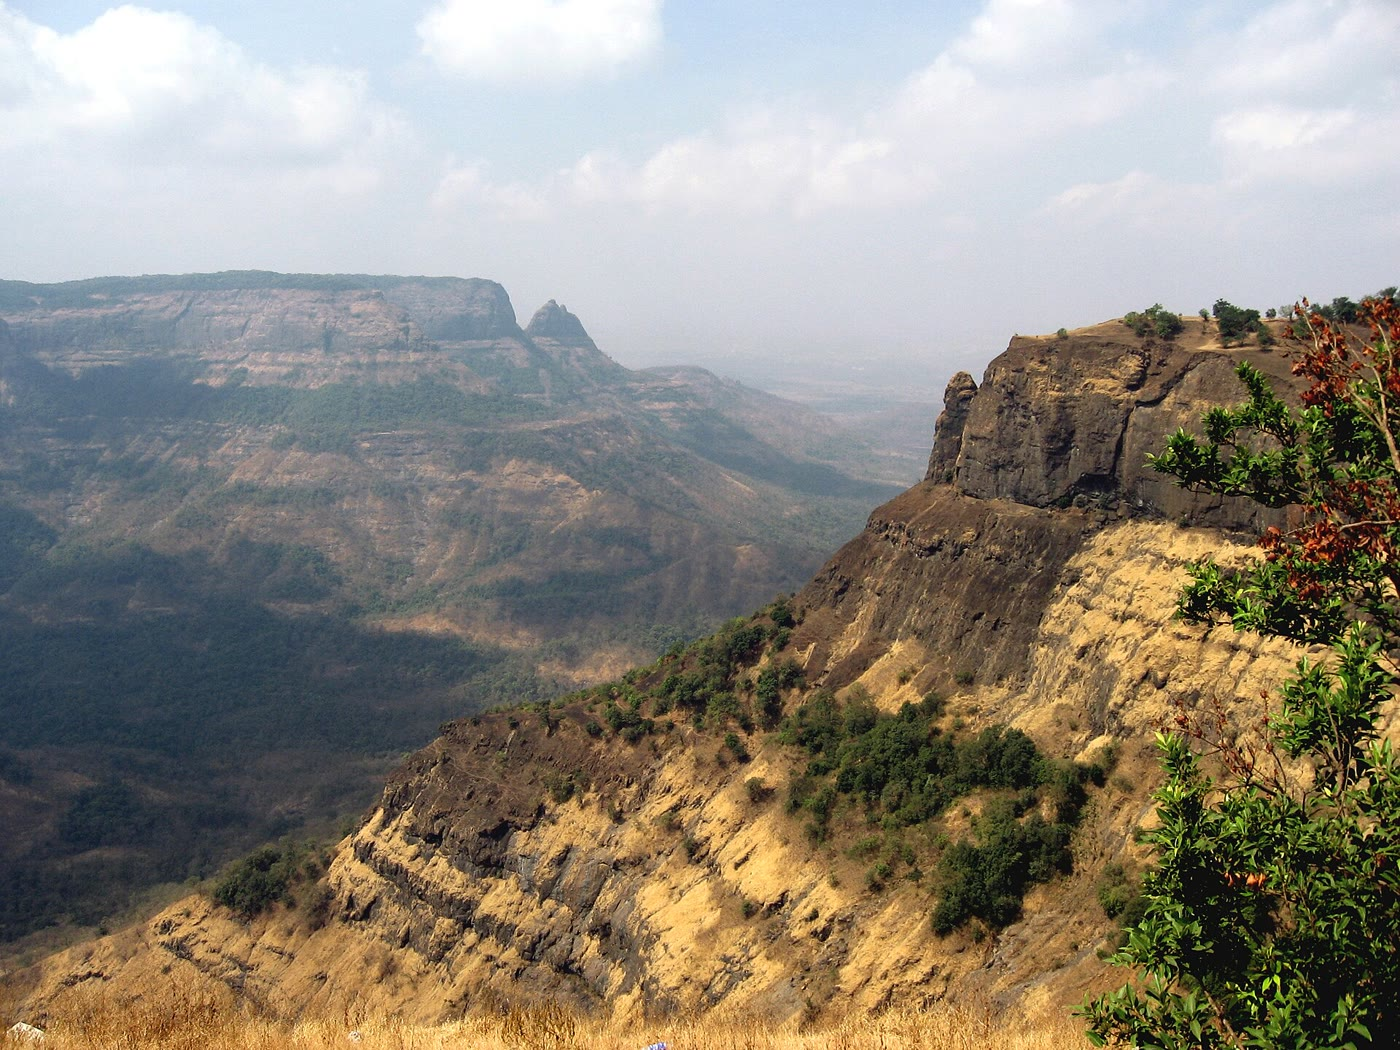
\includegraphics[width=0.55\linewidth]{images/book3/b1-deccan-matheran.jpg}
\par\smallskip{\small The Western Ghats near Matheran, India: flat-topped
hills cut into a pile of nearly horizontal lava flows of the Deccan Traps,
whose resistant layers make the steps of the slopes. Photograph: Nicholas
(Nichalp), CC BY-SA 2.5 (Wikimedia Commons).}
\label{fig:b1:hotspots:deccan}
\end{omfigure}
% ledger: commons:matheran

\begin{center}
\small
\begin{tabular}{llll}
\hline
province & age (Ma) & area (\unit{Mkm^2}) & first volume (\unit{Mkm^3})\\
\hline
Columbia River & 16 & 0.2 & 0.2\\
Ethiopia--Yemen & 30 & 0.7 & 1.2\\
North Atlantic & 61 and 56 & 1.2 & more than 2\\
Deccan & 65.5 & 0.5 (once 1.8) & 2 to 4\\
Ontong Java & 122 and 90 & 2 & 44 (whole \omterm{def:b1:layered-earth:layers}{crust})\\
Paraná--Etendeka & 133 & 1.5 (once over 2) & more than 2.3\\
Karoo--Ferrar & 183 & 3.1 & more than 2.5\\
Central Atlantic (CAMP) & 201 & once up to 7 & more than 2\\
Siberian Traps & 250 & 0.4 (once over 4) & more than 3\\
Emeishan & 259 & 0.5 (once 2 to 5) & more than 1\\
\hline
\end{tabular}
\par\smallskip{\small Mean ages; areas as they are today, and as first
erupted where an estimate exists; volumes of lava as first erupted, except for
the Ontong Java Plateau, whose figure counts its whole thickened \omterm{def:b1:layered-earth:layers}{crust}. Data:
V.~Courtillot and P.~Renne (2003).}
\end{center}
% ledger: cr03:table

\noindent The plume model sketched in \cref{sec:b1:hotspots:plumes} explains both the
size and the haste: a plume head hundreds of kilometres across reaches the base
of the \omterm{def:b1:layered-earth:lithosphere}{lithosphere}, decompresses and melts, and floods the surface; then the
tail goes on building an ordinary \omterm{def:b1:hotspots:track}{hotspot track}. Several provinces are thought
to stand at the old end of a living track: the Deccan Traps and the Réunion
\omterm{def:b1:hotspots:hotspot}{hotspot}, Paraná--Etendeka and Tristan da Cunha, joined by the Walvis Ridge,
and the Columbia River basalts and Yellowstone.
% ledger: cr03:deccan (Reunion hot spot, plume-head model), be08:ojmh (Parana-Etendeka-Walvis-Tristan), pm90:track (Columbia River basalts)

The Deccan Traps of west-central India are a pile of lava flows some
\qty{2500}{m} thick, of which at least \qty{1800}{m} were erupted close to
65.5 million years ago, in much less than a million years; today they cover
about \qty{0.5}{\mega km^2}, perhaps \qty{1.8}{\mega km^2} before erosion. The
Ontong Java Plateau, in the south-western Pacific, is the largest of all
oceanic plateaus: it covers some \qty{2}{\mega km^2}, and its \omterm{def:b1:layered-earth:layers}{crust}, about
\qty{36}{km} thick, holds some \qty{44}{\mega km^3} of igneous rock. The
Manihiki and Hikurangi plateaus, now far apart from it across younger ocean
floor, may have formed with it as a single plateau. The Central Atlantic
Magmatic Province, erupted about 201 million years ago as the Atlantic began to
open, is scattered today, as lavas, dykes and sills, over four continents:
eastern North America, north-eastern South America, West Africa and
south-western Europe; it may once have covered up to \qty{7}{\mega km^2}.
% ledger: cr03:deccan, cr03:table, cr03:ontong-java, be08:ojmh, cr03:camp


Several provinces coincide in time with the great mass extinctions that
biology describes: the Siberian Traps with the largest of all, at the end of
the Permian; the Central Atlantic province with the end of the Triassic; the
Karoo--Ferrar with an extinction in the Early Jurassic; the Emeishan with one
in the Middle Permian; and the Deccan Traps with the end of the Cretaceous. The
four largest extinctions of the last 260 million years each fall, as closely
as the dates can tell, on one of these provinces, and a causal link is
thought the most likely. The proposed mechanisms are atmospheric: sulfate
aerosols that cool the climate for a short time, carbon dioxide that warms it
for much longer, and oceans starved of oxygen. For the end of the Cretaceous,
the Deccan eruptions began before the impact at Chicxulub and went on after
it; a review of the records of the boundary concluded in 2010 that the impact
triggered the extinction.
% ledger: cr03:table, cr03:summary, cr03:deccan, schulte:kpg

Not all volcanism far from plate boundaries needs a plume. Small volcanic
fields grow where a plate is stretched or cracked, and the chains without a
clean \omterm{def:b1:hotspots:track}{age progression} may be fed from the upper \omterm{def:b1:layered-earth:layers}{mantle}; this is the plate
hypothesis at work. What the oceanic islands become after the \omterm{def:b1:hotspots:hotspot}{hotspot} has left
them, as they sink, wear down and grow reefs, belongs to the Year 2 volume.
% ledger: fn03:plate-hypothesis

\section{Exercises}

\begin{exercise}[$\star$]\label{exo:b1:hotspots:1}
(a) Mauna Kea rises \qty{4205}{m} above sea level, and the sea floor far from
the Hawaiian chain lies \qty{5274}{m} deep. How high does the volcano stand
above that floor? Why is its true height from its base greater still?
(b) Mauna Loa holds about \qty{74000}{km^3}. How long would it take to build
at Kilauea's present supply, \qty{0.1}{km^3} a year, and at the mean rate of
the whole chain, \qty{0.025}{km^3} a year? (c) The Pu\textquoteleft
u~\textquoteleft O\textquoteleft o eruption poured out about \qty{0.12}{km^3}
a year from 1983 to 2002. What volume is that, and what fraction of Mauna Loa?
% ledger: pp1801:volumes, pp1801:kilauea-supply, pp1801:chain-volume, pp1801:kilauea-rate; 5274 m from hotspots.py
\end{exercise}

\begin{exercise}[$\star$]\label{exo:b1:hotspots:2}
A plate turns over the \omterm{def:b1:hotspots:hotspot}{hotspots} at \qty{0.92}{\degree\per\Myr}. Take
$R = \qty{6371}{km}$. (a) Express $\omega$ in radians per million years. (b)
Compute the speed, in \unit{mm.yr^{-1}}, of \omterm{def:b1:hotspots:hotspot}{hotspots} \ang{30}, \ang{60},
\ang{90} and \ang{108.0} from the pole. (c) Why is the speed of Hawaii, at
\ang{108.0}, less than at \ang{90}?
\end{exercise}

\begin{exercise}[$\star$]\label{exo:b1:hotspots:3}
(a) Compute the mean thickness of the Deccan Traps as they are today,
\qty{1}{\mega km^3} over \qty{0.5}{\mega km^2}, and of the Central Atlantic
province, \qty{2}{\mega km^3} over \qty{7}{\mega km^2}. (b) Compare with the
thickness of the Deccan section, \qty{2500}{m}. (c) Why does the mean
thickness of the Central Atlantic province say little about the thickness of
its lava piles?
% ledger: cr03:table, cr03:deccan, cr03:camp
\end{exercise}

\begin{exercise}[$\star$]\label{exo:b1:hotspots:4}
Plume rock \qty{250}{K} hotter than the \omterm{def:b1:layered-earth:layers}{mantle} around it has
$\alpha = \qty{3.2e-5}{K^{-1}}$ and $\rho_m = \qty{3300}{kg.m^{-3}}$. (a) By how
much is it lighter, in \unit{kg.m^{-3}}? (b) What thickness of such rock,
spread beneath the plate, would hold up isostatically a swell \qty{690}{m}
high under the sea ($\rho_w = \qty{1000}{kg.m^{-3}}$)?
% ledger: herzberg:tp (200-300 K), parsons:plate-model (alpha)
\end{exercise}

\begin{exercise}[$\star\star$]\label{exo:b1:hotspots:5}
Two \omterm{def:b1:hotspots:hotspot}{hotspots} lie on the equator, A at \ang{0}\,E and B at \ang{90}\,E, and
both tracks run due west (\omterm{def:b1:spherical-astronomy:horizontal}{azimuth} \ang{270}). (a) Compute the track vectors
$\vec t_A$ and $\vec t_B$. (b) Compute $\vec t_A\times\vec t_B$. (c) Apply the
sign rule of \cref{prop:b1:hotspots:two-tracks}: where is the \omterm{def:b1:plate-kinematics:euler-pole}{Euler pole}?
Explain the result without computation. (d) If A moves at \qty{50}{mm.yr^{-1}},
what is $\omega$ in degrees per million years?
\end{exercise}

\begin{exercise}[$\star\star$]\label{exo:b1:hotspots:6}
Three \omterm{def:b1:hotspots:hotspot}{hotspots} of one plate lie at the distances $x = R\sin\Delta = 3000$, 5000
and \qty{6000}{km} from the axis of rotation and move at 30, 48 and
\qty{57}{mm.yr^{-1}}. (a) Fit $v = \omega x$ by least squares and give
$\omega$ in radians and in degrees per million years. (b) Compute the
residuals. (c) Why must the line pass through the origin?
\end{exercise}

\begin{exercise}[$\star\star$]\label{exo:b1:hotspots:7}
A swell of cross-section \qty{3e8}{m^2} surrounds a \omterm{def:b1:hotspots:track}{hotspot track} on a plate
moving at \qty{50}{mm.yr^{-1}}. Take $\rho_m - \rho_w = \qty{2300}{kg.m^{-3}}$,
$c_p = \qty{910}{J.kg^{-1}.K^{-1}}$ and $\alpha = \qty{3.2e-5}{K^{-1}}$. (a)
Compute its buoyancy flux and its heat flux. (b) Compare with Hawaii,
\qty{3240}{kg.s^{-1}}. (c) Two \omterm{def:b1:hotspots:hotspot}{hotspots} have the same swell; one lies under a
plate moving twice as fast. Which plume is stronger?
\end{exercise}

\begin{exercise}[$\star\star$]\label{exo:b1:hotspots:8}
Along the Yellowstone track, the caldera eruptions began in the McDermitt
volcanic field 16.1 million years ago and in the Picabo field, some
\qty{350}{km} to the north-east, 10.3 million years ago; since then they have
moved at $\qty[uncertainty-mode=separate]{2.9 \pm 0.5}{cm}$ a year towards
N\,\ang{54}\,E. (a) At what mean speed did the volcanism migrate from McDermitt
to Picabo? (b) Compare both speeds with that of the plate over the \omterm{def:b1:hotspots:hotspot}{hotspot},
\qty[uncertainty-mode=separate]{26 \pm 5}{mm.yr^{-1}} towards \ang{235}. (c) Is
the direction of the young track the one expected? (d) The older part of the
track lies in a region that has been stretched as the volcanism passed. How
can this explain the difference?
% ledger: pm90:track, data:b3-hotspots
\end{exercise}

\begin{exercise}[$\star\star$]\label{exo:b1:hotspots:9}
The Hawaiian plume carries about \qty{9.2e10}{W} of excess heat. (a) If all of
it left through the \qty{1000}{km} by \qty{1000}{km} of sea floor nearest the
\omterm{def:b1:hotspots:hotspot}{hotspot}, by how much would the \omterm{def:b1:heat-budget:heat-flow}{heat flow} there be raised? (b) Compare with the
observed excess, at most 5 to \qty{10}{mW.m^{-2}}. (c) How long does heat take to
diffuse through a plate \qty{100}{km} thick ($\kappa = \qty{e-6}{m^2.s^{-1}}$)?
How long does the plate take to cross \qty{1000}{km} at \qty{92}{mm.yr^{-1}}?
Conclude.
% ledger: vh89:swell-heat
\end{exercise}

\begin{exercise}[$\star\star\star$]\label{exo:b1:hotspots:10}
The Deccan Traps hold about \qty{e6}{km^3} of lava. Suppose it came from a
spherical plume head of which one tenth melted. (a) What was the volume and
the radius of the head? (b) Flattened beneath the \omterm{def:b1:layered-earth:lithosphere}{lithosphere} into a disc
\qty{100}{km} thick, what diameter would the head have? Compare its area with
the area the Traps may once have covered, \qty{1.8}{\mega km^2}. (c) If the
lava was erupted in one million years, compare its rate with the present
supply of Kilauea, \qty{0.1}{km^3} a year. (d) Why must a plume head be large,
while the tail that follows is narrow?
% ledger: cr03:table, pp1801:kilauea-supply
\end{exercise}

\begin{exercise}[$\star\star\star$]\label{exo:b1:hotspots:11}
Between 81 and 47 million years ago the Hawaiian \omterm{def:b1:hotspots:hotspot}{hotspot} moved south at more
than \qty{40}{mm.yr^{-1}}. (a) Taking \qty{40}{mm.yr^{-1}}, how far did it
move?
(b) Suppose the plate moved meanwhile at \qty{80}{mm.yr^{-1}} towards
\ang{340} over the deep \omterm{def:b1:layered-earth:layers}{mantle}. With $x$ east and $y$ north, compute the
velocity of the plate relative to the drifting \omterm{def:b1:hotspots:hotspot}{hotspot}, its speed and its
\omterm{def:b1:spherical-astronomy:horizontal}{azimuth}. (c) By what percentage, and by how many degrees, would a track built
then misrepresent the motion of the plate over the deep \omterm{def:b1:layered-earth:layers}{mantle}?
% ledger: tarduno:emperor
\end{exercise}

\begin{exercise}[$\star\star\star$]\label{exo:b1:hotspots:12}
(a) A flood basalt of \qty{e6}{km^3} cools from about \qty{1300}{\celsius} to
the temperature of the surface. With a heat capacity of \qty{3}{MJ.m^{-3}.K^{-1}},
how much heat does it give out (ignore the latent heat of crystallisation)?
(b) Spread over one million years, what power is that? Compare with the
Hawaiian plume, \qty{9.2e10}{W}, and with the \qty{47}{TW} of the whole Earth.
(c) A plume head also heats the base of the \omterm{def:b1:layered-earth:lithosphere}{lithosphere} without melting all of
it. Is the power of (b) an upper or a lower bound for the heat brought by the
head?
% ledger: delaney86:properties (Book 2 row, 2-3 MJ/m3/K), dd10:total; 1300 degC is an exercise value
\end{exercise}

\section{Problem: The Pacific plate's speedometer}

\begin{problem}[{Weekend problem --- the Euler pole of the Pacific plate from two
hotspot tracks, its rate from a third measurement, a test on other hotspots,
and the Hawaiian plume's buoyancy and supply}]
\label{pb:b1:hotspots:1}
% values: calc/ch15.py; ledger: data:b3-hotspots, data:etopo1, pp1801:kilauea-supply, pp1801:volumes,
% pp1801:chain-volume, delaney86:properties, parsons:plate-model, dd10:total, data:pb2002 (ridge_budget.py), cd87:rate
Morgan and Morgan list the Hawaiian \omterm{def:b1:hotspots:hotspot}{hotspot} at \ang{19.0}\,N, \ang{155.2}\,W,
with a track towards $\ang{304}\pm\ang{3}$ and a speed of
\qty[uncertainty-mode=separate]{92 \pm 3}{mm.yr^{-1}}, and the Louisville
\omterm{def:b1:hotspots:hotspot}{hotspot} at \ang{53.6}\,S, \ang{140.6}\,W, with a track towards $\ang{316}\pm\ang{5}$
and a speed of \qty[uncertainty-mode=separate]{67 \pm 5}{mm.yr^{-1}}. Use the
axes and the vectors $\vec e$, $\vec n$, $\vec t$ of
\cref{sec:b1:hotspots:tracks}, with $R = \qty{6371}{km}$. Give components to
four decimals.

\medskip
\noindent\textbf{Part I --- The pole from two tracks.}
\begin{enumerate}
  \item Compute $\vec r$, $\vec e$ and $\vec n$ at Hawaii, then the track
        vector $\vec t_H$.
  \item Do the same at Louisville: $\vec r_L$, $\vec e$, $\vec n$ and
        $\vec t_L$.
  \item Check that $\vec t_H$ is a unit vector perpendicular to $\vec r_H$.
  \item Compute $\vec t_H\times\vec t_L$ and its length. What angle do the two
        track vectors make?
  \item Normalise the cross product and apply the sign rule of
        \cref{prop:b1:hotspots:two-tracks}.
  \item Give the \omterm{def:b1:spherical-astronomy:geographic}{latitude} and \omterm{def:b1:spherical-astronomy:geographic}{longitude} of the \omterm{def:b1:plate-kinematics:euler-pole}{Euler pole} of the Pacific plate
        relative to the \omterm{def:b1:hotspots:hotspot}{hotspots}.
\end{enumerate}

\medskip
\noindent\textbf{Part II --- The rate.}
\begin{enumerate}[resume]
  \item Compute the angular distances $\Delta_H$ and $\Delta_L$ from the pole
        to the two \omterm{def:b1:hotspots:hotspot}{hotspots}.
  \item Compute $(\vec p\times\vec r_L)\cdot\vec t_L$. Explain why it equals
        $\sin\Delta_L$, and what its sign says about the motion at Louisville.
  \item From the speed at Louisville, compute $\omega$ in radians and in
        degrees per million years.
  \item How long does the Pacific plate take to make a full turn about this
        pole?
  \item The least-squares pole of the fifteen Pacific tracks lies at
        \ang{63.78}\,S, \ang{112.48}\,E, with \qty{0.92}{\degree\per\Myr}.
        Compute the angle between the two poles and compare the two rates.
\end{enumerate}

\medskip
\noindent\textbf{Part III --- A test on three more hotspots.} Morgan and
Morgan give the Society \omterm{def:b1:hotspots:hotspot}{hotspot} (\ang{18.2}\,S, \ang{148.4}\,W)
\qty[uncertainty-mode=separate]{109 \pm 10}{mm.yr^{-1}}, Pitcairn
(\ang{25.4}\,S, \ang{129.3}\,W)
\qty[uncertainty-mode=separate]{90 \pm 15}{mm.yr^{-1}} and Cobb
(\ang{46.0}\,N, \ang{130.1}\,W)
\qty[uncertainty-mode=separate]{43 \pm 3}{mm.yr^{-1}}.
\begin{enumerate}[resume]
  \item Compute the angular distance from the pole of question 6 to each of the
        three \omterm{def:b1:hotspots:hotspot}{hotspots}.
  \item Predict the three speeds with the rate of question 9.
  \item Which predictions agree with the measured speeds within their
        uncertainties, and which do not?
  \item Two tracks of different directions always give a pole. Why are two
        tracks that are nearly parallel a poor choice?
\end{enumerate}

\medskip
\noindent\textbf{Part IV --- The plume and the speedometer.} The Hawaiian swell
has the cross-section \qty{4.83e8}{m^2}. Take
$\rho_m - \rho_w = \qty{2300}{kg.m^{-3}}$, $c_p = \qty{910}{J.kg^{-1}.K^{-1}}$
and $\alpha = \qty{3.2e-5}{K^{-1}}$.
\begin{enumerate}[resume]
  \item Convert \qty{92}{mm.yr^{-1}} to \unit{m.s^{-1}} and compute the
        buoyancy flux of the Hawaiian plume.
  \item Compute the excess heat it carries, and compare with the \qty{47}{TW}
        that leave the Earth.
  \item The ridges make about \qty{21}{km^3} of \omterm{def:b1:layered-earth:layers}{crust} a year along some
        \qty{67000}{km}. What length of ridge makes as much \omterm{def:b1:layered-earth:layers}{crust} as Kilauea
        is supplied with, \qty{0.1}{km^3} a year?
  \item At that rate, how long would Mauna Loa, about \qty{74000}{km^3},
        take to grow?
  \item The \omterm{def:b1:hotspots:hotspot}{hotspot} built about \qty{2e6}{km^3} of the chain in 81 million
        years. Compute its mean output and compare with Kilauea's supply today.
  \item With the pole and the rate of Parts I and II, compute the speed that
        the Louisville track predicts for the Pacific plate over the Hawaiian
        \omterm{def:b1:hotspots:hotspot}{hotspot}.
  \item Compare with the measured \qty[uncertainty-mode=separate]{92 \pm 3}{mm.yr^{-1}}: by how much, and
        by how many standard uncertainties, do they differ?
  \item From the ages of the Hawaiian volcanoes, Book 2 found \qty{9.1}{cm} a
        year, and the authors of the ages, fitting the whole chain,
        \qty{8.6}{cm} a year. Compare these averages over tens of millions of
        years with the two \omterm{def:b1:hotspots:hotspot}{hotspot} speeds.
  \item To one decimal, in centimetres a year, what speed does the Louisville
        track give the Pacific plate over the Hawaiian \omterm{def:b1:hotspots:hotspot}{hotspot}?
\end{enumerate}
\end{problem}
